\documentclass[10pt,a4paper]{article}
\usepackage[margin=2cm,headheight=14pt]{geometry}
\usepackage[T1]{fontenc}
\usepackage{needspace,xcolor,booktabs,array,enumitem,hyperref,fancyhdr,graphicx}
\usepackage{listings}
\usepackage[most]{tcolorbox}
\usepackage{tikz}
\usetikzlibrary{arrows.meta,positioning,shapes.geometric,fit,backgrounds}

\definecolor{cane}{HTML}{2E7D32}
\definecolor{caneL}{HTML}{E8F3E4}
\definecolor{ink}{HTML}{1D2B1A}
\definecolor{warn}{HTML}{B26A00}
\hypersetup{colorlinks=true,linkcolor=cane,urlcolor=cane}
\setlist{itemsep=2pt,topsep=3pt}
\pagestyle{fancy}\fancyhf{}
\lhead{\small ML DevOps Laboratory (UDSPC0732) --- ISE-2}
\rhead{\small CaneCCS-MLOps}
\cfoot{\small\thepage}
\renewcommand{\headrulewidth}{0.4pt}

\lstdefinestyle{code}{basicstyle=\ttfamily\scriptsize,backgroundcolor=\color{gray!8},frame=single,
 rulecolor=\color{gray!50},breaklines=true,showstringspaces=false,numbers=left,numberstyle=\tiny\color{gray},
 numbersep=5pt,keywordstyle=\color{cane}\bfseries,commentstyle=\color{gray},xleftmargin=12pt,columns=fullflexible}
\lstset{style=code}

\newtcolorbox{note}[1][]{colback=caneL,colframe=cane,fonttitle=\bfseries,title=#1,boxrule=0.6pt,arc=2pt,left=4pt,right=4pt,top=3pt,bottom=3pt}
\newtcolorbox{shot}[1]{colback=white,colframe=warn,boxrule=0.8pt,arc=2pt,enhanced,frame style={dashed},height=3.1cm,valign=center,halign=center,
 title={\small Screenshot to paste: #1},fonttitle=\bfseries\small,coltitle=warn,colbacktitle=white}

\usepackage{titlesec}
\titleformat{\section}{\large\bfseries\color{cane}}{\thesection.}{0.5em}{}[\vspace{-6pt}\color{cane}\rule{\linewidth}{0.5pt}]
\titleformat{\subsection}{\normalsize\bfseries\color{ink}}{\thesubsection}{0.5em}{}
\titlespacing*{\section}{0pt}{10pt}{6pt}

\let\oldsection\section
\renewcommand{\section}{\Needspace{14\baselineskip}\oldsection}
\begin{document}

\begin{tcolorbox}[colback=cane,colframe=cane,coltext=white,arc=3pt,left=10pt,right=10pt,top=8pt,bottom=8pt]
{\Large\bfseries CaneCCS-MLOps}\\[2pt]
{\large An MLOps use case: CI/CD pipeline and monitoring for sugarcane CCS prediction}\\[6pt]
\small ISE-2 \textbullet\ ML DevOps Laboratory (UDSPC0732) \textbullet\ Academic Year 2026--27
\end{tcolorbox}

\vspace{4pt}
\begin{tabular}{@{}p{0.15\linewidth}p{0.31\linewidth}p{0.17\linewidth}p{0.27\linewidth}@{}}
\textbf{Name} & Niranjan & \textbf{PRN} & 2324000035\\
\textbf{Course} & ML DevOps Laboratory & \textbf{Course Code} & UDSPC0732\\
\textbf{Assessment} & ISE-2 (10 marks) & \textbf{COs covered} & CO1 (L2), CO4 (L4)\\
\textbf{Tools} & Python, Flask, Git, GitHub, Jenkins, Docker, Prometheus, Grafana & \textbf{Date} & 29 October 2026\\
\end{tabular}

%---------------------------------------------------------------
\section{Problem statement}
Sugar mills pay farmers according to the \textbf{Commercial Cane Sugar (CCS \%)} of each delivered batch, but the
laboratory value is available only hours after the truck is unloaded. Cane also loses sugar every day it waits between
harvest and crushing (field-to-mill delay), which is a recurring source of disputes in Maharashtra's sugar belt.

\textbf{Goal.} Build a small ML web service that estimates CCS \% from fast weighbridge readings (brix, pol, fibre \%,
trash \%, days since harvest, cane variety), and wrap it in a complete \textbf{CI/CD and monitoring} workflow so that every
code change is tested, containerised, deployed and observed automatically.

\begin{note}[Why this niche use case?]
Most lab projects deploy a generic Iris or house-price model. Here the model is deliberately domain-specific
(sugarcane agronomy), and the monitoring is domain-aware: it tracks \emph{brix drift} (a change in incoming cane quality, e.g.\ after
a bad monsoon) and \emph{low-CCS batches}, not just HTTP errors. This is what separates ML monitoring from ordinary
web monitoring.
\end{note}

\subsection*{Mapping to course outcomes}
\begin{tabular}{@{}p{0.12\linewidth}p{0.82\linewidth}@{}}
\toprule
\textbf{CO1 (L2)} & Explain and configure the DevOps toolchain: Git, GitHub, Jenkins, Docker, and how they fit the ML lifecycle (Sections 4--8).\\
\textbf{CO4 (L4)} & Analyse a deployed ML service using monitoring tools: metrics design, dashboards, alert rules, drift signal (Sections 9--11).\\
\bottomrule
\end{tabular}

%---------------------------------------------------------------
\section{Model and data}
\textbf{Model:} \texttt{GradientBoostingRegressor} (scikit-learn) predicting CCS \%.
\textbf{Inputs:} brix, pol, fibre \%, trash \%, days since harvest, variety (Co-86032, CoM-0265, Co-0238).

\textbf{Data.} A real mill dataset is proprietary, so \texttt{train.py} generates \textbf{synthetic} lab records (6{,}000 rows)
from the standard Indian CCS relation $\mathrm{CCS}_{juice}=0.73\,[\,\mathrm{pol}-0.4(\mathrm{brix}-\mathrm{pol})\,]$, corrected for fibre and
trash, a field-to-mill sugar-loss term (about 0.28\,\% per day, increasing with delay), a small variety effect and noise.
The focus of this assignment is the \emph{pipeline}, not model novelty, and this is disclosed so results are not mistaken for field data.

\begin{center}
\begin{tabular}{lll}
\toprule
\textbf{Metric (20\% hold-out)} & \textbf{Value} & \textbf{Train rows}\\
\midrule
MAE & 0.118 CCS points & 4{,}800\\
$R^2$ & 0.9855 & \\
\bottomrule
\end{tabular}
\end{center}

%---------------------------------------------------------------
\section{System architecture}
\begin{center}
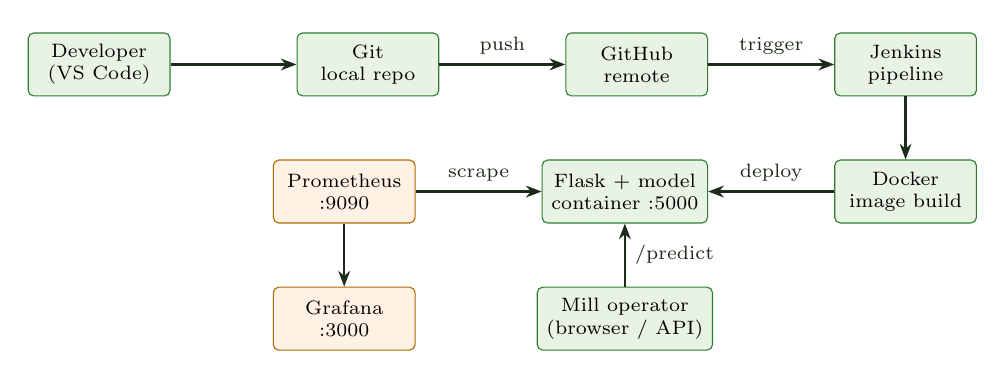
\begin{tikzpicture}[font=\scriptsize,node distance=8mm and 16mm,
 box/.style={draw=cane,fill=caneL,rounded corners=2pt,minimum height=8mm,minimum width=18mm,align=center},
 mon/.style={draw=warn,fill=orange!10,rounded corners=2pt,minimum height=8mm,minimum width=18mm,align=center},
 arr/.style={-{Stealth[length=2mm]},thick,color=ink}]
\node[box] (dev) {Developer\\(VS Code)};
\node[box,right=of dev] (git) {Git\\local repo};
\node[box,right=of git] (gh) {GitHub\\remote};
\node[box,right=of gh] (jen) {Jenkins\\pipeline};
\node[box,below=of jen] (dock) {Docker\\image build};
\node[box,left=of dock] (app) {Flask + model\\container :5000};
\node[mon,left=of app] (prom) {Prometheus\\:9090};
\node[mon,below=of prom] (graf) {Grafana\\:3000};
\node[box,below=of app] (user) {Mill operator\\(browser / API)};
\draw[arr] (dev)--(git); \draw[arr] (git)--node[above]{push}(gh); \draw[arr] (gh)--node[above]{trigger}(jen);
\draw[arr] (jen)--(dock); \draw[arr] (dock)--node[above]{deploy}(app);
\draw[arr] (user)--node[right]{/predict}(app);
\draw[arr] (prom)--node[above]{scrape}(app);
\draw[arr] (prom)--(graf);
\end{tikzpicture}
\end{center}

%---------------------------------------------------------------
\section{Tools: installation and verification}
\begin{center}
\small
\begin{tabular}{@{}p{0.16\linewidth}p{0.26\linewidth}p{0.45\linewidth}@{}}
\toprule
\textbf{Tool} & \textbf{Role in this project} & \textbf{Verification command}\\
\midrule
Python 3.12 & runtime for training and Flask & \texttt{python --version}\\
Flask 3.1 & web/API layer & \texttt{python -c "import flask;print(flask.\_\_version\_\_)"}\\
Git & version control & \texttt{git --version}\\
GitHub & remote repo, webhook source & \texttt{git remote -v}\\
Docker Desktop & containerisation & \texttt{docker --version \&\& docker run hello-world}\\
Jenkins (LTS) & CI/CD orchestration & open \texttt{http://localhost:8080}\\
Prometheus & metrics collection & open \texttt{http://localhost:9090/targets}\\
Grafana & dashboards & open \texttt{http://localhost:3000}\\
\bottomrule
\end{tabular}
\end{center}

\begin{shot}{terminal showing python, git and docker version outputs}\end{shot}
\vspace{4pt}
\begin{shot}{Jenkins login page / dashboard at localhost:8080 (after unlock + suggested plugins)}\end{shot}

\begin{note}[Jenkins setup checklist]
\begin{enumerate}[leftmargin=14pt]
\item Run Jenkins (Windows installer, or \texttt{docker run -p 8080:8080 -v jenkins\_home:/var/jenkins\_home jenkins/jenkins:lts}).
\item Unlock with the initial admin password, install \emph{suggested plugins}, add \emph{Pipeline}, \emph{Git}, \emph{GitHub} and \emph{JUnit} if missing.
\item Make sure the Jenkins user can run \texttt{docker} and \texttt{python} (Windows: add both to the system PATH and restart the Jenkins service).
\end{enumerate}
\end{note}

%---------------------------------------------------------------
\section{Flask application}
\textbf{Project layout}
\begin{lstlisting}[numbers=none]
canesugar-mlops/
|-- app/main.py              # Flask API + Prometheus metrics
|-- app/templates/index.html # prediction form
|-- train.py                 # trains and saves model + meta.json
|-- tests/test_app.py        # 6 pytest unit tests
|-- Dockerfile  docker-compose.yml  Jenkinsfile
|-- prometheus/{prometheus.yml, alerts.yml}
`-- grafana/{provisioning/, dashboards/cane.json}
\end{lstlisting}

\textbf{Endpoints}\\[2pt]
\begin{tabular}{@{}lll@{}}
\toprule
\texttt{GET /} & HTML form & operator UI\\
\texttt{POST /predict} & JSON $\rightarrow$ \{ccs, grade\} & validates input, returns 400 on bad data\\
\texttt{GET /health} & liveness probe & used by Docker and Jenkins smoke test\\
\texttt{GET /model-info} & model metadata & version, MAE, $R^2$\\
\texttt{GET /metrics} & Prometheus exposition & scraped every 5 s\\
\bottomrule
\end{tabular}

\subsection*{app/main.py}
\lstinputlisting[language=Python]{../app/main.py}

\begin{shot}{browser at localhost:5000 showing the prediction form with a result}\end{shot}

%---------------------------------------------------------------
\section{Git and GitHub}
\begin{lstlisting}[language=bash,numbers=none]
git init
git add .
git commit -m "Initial commit: CaneCCS MLOps pipeline"
git branch -M main
git remote add origin https://github.com/<your-username>/canesugar-mlops.git
git push -u origin main
\end{lstlisting}
Branch workflow used: feature branch $\rightarrow$ pull request $\rightarrow$ merge to \texttt{main}; the merge triggers Jenkins.
A lightweight GitHub Actions workflow (\texttt{.github/workflows/ci.yml}) also runs training and tests on every push as a second, cloud-side check.

\begin{shot}{GitHub repository page showing the project files and commit history}\end{shot}

%---------------------------------------------------------------
\section{Docker}
\lstinputlisting[language=bash,caption={\small Dockerfile}]{../Dockerfile}
\vspace{-2pt}
\lstinputlisting[caption={\small docker-compose.yml (app + Prometheus + Grafana)}]{../docker-compose.yml}

\begin{note}[Design choice: one gunicorn worker with threads]
\texttt{prometheus\_client} keeps counters in process memory. With two gunicorn workers each worker reports its own
numbers, so Prometheus sees values jump between workers. The container therefore uses \texttt{-w 1 --threads 4},
which keeps all metrics in one process (see Section 11).
\end{note}

\begin{shot}{terminal: docker compose up -d --build, then docker ps showing 3 containers}\end{shot}

%---------------------------------------------------------------
\section{Jenkins CI/CD pipeline}
\begin{center}
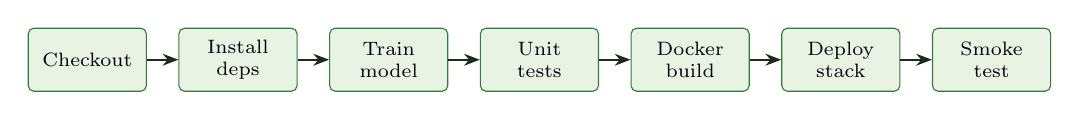
\begin{tikzpicture}[font=\scriptsize,node distance=4mm,
 st/.style={draw=cane,fill=caneL,rounded corners=2pt,minimum height=8mm,minimum width=15mm,align=center},
 arr/.style={-{Stealth[length=2mm]},thick,color=ink}]
\node[st] (a) {Checkout};
\node[st,right=of a] (b) {Install\\deps};
\node[st,right=of b] (c) {Train\\model};
\node[st,right=of c] (d) {Unit\\tests};
\node[st,right=of d] (e) {Docker\\build};
\node[st,right=of e] (f) {Deploy\\stack};
\node[st,right=of f] (g) {Smoke\\test};
\foreach \x/\y in {a/b,b/c,c/d,d/e,e/f,f/g}{\draw[arr](\x)--(\y);}
\end{tikzpicture}
\end{center}
The pipeline is a \emph{declarative} Jenkinsfile stored in the repository (pipeline-as-code). If tests fail the build stops, so a broken model never reaches the Docker stage.

\textbf{Creating the job:} New Item $\rightarrow$ \emph{Pipeline} $\rightarrow$ Definition: \emph{Pipeline script from SCM} $\rightarrow$ SCM: Git $\rightarrow$
repository URL $\rightarrow$ branch \texttt{*/main} $\rightarrow$ script path \texttt{Jenkinsfile}. Under \emph{Build Triggers} enable
\emph{GitHub hook trigger} (or \emph{Poll SCM} with \texttt{H/2 * * * *} when Jenkins is not publicly reachable).

\lstinputlisting[language=Java,caption={\small Jenkinsfile}]{../Jenkinsfile}

\begin{shot}{Jenkins job configuration page (Pipeline script from SCM)}\end{shot}
\vspace{4pt}
\begin{shot}{Jenkins Stage View with all stages green}\end{shot}
\vspace{4pt}
\begin{shot}{Jenkins Console Output ending with ``Finished: SUCCESS''}\end{shot}

%---------------------------------------------------------------
\section{Monitoring: Prometheus and Grafana}
\subsection*{Metrics exposed by the application}
\begin{center}
\small
\begin{tabular}{@{}p{0.42\linewidth}p{0.11\linewidth}p{0.40\linewidth}@{}}
\toprule
\textbf{Metric} & \textbf{Type} & \textbf{Why it matters}\\
\midrule
\texttt{cane\_http\_requests\_total\{endpoint,status\}} & Counter & traffic and error ratio\\
\texttt{cane\_request\_latency\_seconds} & Histogram & p95 latency SLO\\
\texttt{cane\_predictions\_total} & Counter & throughput\\
\texttt{cane\_prediction\_errors\_total} & Counter & bad client input\\
\texttt{cane\_predicted\_ccs} & Histogram & prediction distribution (output drift)\\
\texttt{cane\_brix\_drift\_zscore} & Gauge & rolling mean brix of last 50 requests vs.\ training mean, in std units (input drift)\\
\texttt{cane\_low\_ccs\_batches\_total} & Counter & business signal: batches predicted below 9 CCS\\
\texttt{cane\_model\_info} & Gauge & which model version is live\\
\bottomrule
\end{tabular}
\end{center}

\lstinputlisting[language=bash,caption={\small prometheus/prometheus.yml}]{../prometheus/prometheus.yml}
\vspace{-2pt}
\lstinputlisting[caption={\small prometheus/alerts.yml}]{../prometheus/alerts.yml}

\subsection*{Grafana}
Grafana is \emph{provisioned as code}: the data source (\texttt{grafana/provisioning/datasources/ds.yml}) and a six-panel dashboard
(\texttt{grafana/dashboards/cane.json}) load automatically at start-up, so the monitoring view is reproducible and not hand-built.
Login \texttt{admin/admin} at \texttt{localhost:3000}, dashboard \emph{CaneCCS ML Monitoring}.

\begin{center}\small
\begin{tabular}{@{}p{0.25\linewidth}p{0.68\linewidth}@{}}
\toprule
\textbf{Panel} & \textbf{PromQL}\\
\midrule
Predictions per minute & \texttt{rate(cane\_predictions\_total[1m])*60}\\
p95 predict latency & \texttt{histogram\_quantile(0.95,}\newline \texttt{\ \ sum(rate(cane\_request\_latency\_seconds\_bucket}\newline \texttt{\ \ \{endpoint="predict"\}[1m])) by (le))}\\
Brix drift (z-score) & \texttt{cane\_brix\_drift\_zscore}\\
Invalid requests / min & \texttt{rate(cane\_prediction\_errors\_total[1m])*60}\\
\bottomrule
\end{tabular}
\end{center}

\begin{shot}{Prometheus Status $\rightarrow$ Targets page showing cane-app as UP}\end{shot}
\vspace{4pt}
\begin{shot}{Grafana dashboard ``CaneCCS ML Monitoring'' with live panels}\end{shot}

%---------------------------------------------------------------
\section{Testing and results}
\subsection*{Unit tests (pytest)}
\lstinputlisting[numbers=none]{evidence/pytest.txt}

\subsection*{API calls against the running service}
\lstinputlisting[numbers=none]{evidence/curl.txt}

Observations: the same cane (brix 19.5, pol 17.2) predicts 9.61 CCS when one day old (grade B) but a different variety held five days
drops to 8.58 (grade C), reproducing the field-to-mill loss the model was built to capture. Invalid input (pol greater than brix) is rejected with HTTP 400.

\subsection*{Drift experiment}
After normal traffic I sent 30 high-brix batches (brix 23.5, against a training mean of 19.5). The service then exposed:
\lstinputlisting[numbers=none]{evidence/metrics.txt}
The brix drift z-score of about 2.3 exceeds the 1.5 threshold in \texttt{alerts.yml}, so the \texttt{BrixInputDrift} alert would fire
after 30 s, signalling that the input distribution has moved away from what the model was trained on and retraining should be considered.

%---------------------------------------------------------------
\section{Problems faced and how they were solved}
\begin{enumerate}[leftmargin=14pt]
\item \textbf{Metrics did not add up.} 32 valid predictions were sent but \texttt{/metrics} showed 18. Cause: gunicorn ran two worker processes, each with its own in-memory counters.
 Fix: one worker with four threads (\texttt{-w 1 --threads 4}); afterwards the counters matched exactly (32 predictions, 1 error).
\item \textbf{Windows vs.\ Linux Jenkins agents.} \texttt{sh} fails on Windows agents. The Jenkinsfile uses \texttt{isUnix()} to pick \texttt{sh} or \texttt{bat}.
\item \textbf{Model missing in a fresh clone.} The \texttt{.joblib} file is git-ignored, so the pipeline (and Dockerfile) retrain it with \texttt{train.py}, keeping the repository small and builds reproducible.
\item \textbf{Grade thresholds.} Initial A/B/C cut-offs never produced grade A on realistic inputs; they were recalibrated against the model's output range.
\end{enumerate}

%---------------------------------------------------------------
\section{Conclusion}
The project delivers a niche, domain-specific ML service together with a full DevOps loop: code in Git/GitHub, an automated Jenkins pipeline that trains, tests, builds and deploys a Docker image,
and a Prometheus/Grafana stack that watches both system health and ML-specific signals (input drift, prediction distribution, low-quality batches).
Future work: multiprocess Prometheus mode for horizontal scaling, Alertmanager e-mail/Slack notifications, model registry (MLflow) and a scheduled retraining job triggered by the drift alert.

\subsection*{References}
\begin{itemize}[leftmargin=14pt]\small
\item Flask docs: \url{https://flask.palletsprojects.com} \quad Jenkins docs: \url{https://www.jenkins.io/doc/book/pipeline/}
\item Docker docs: \url{https://docs.docker.com} \quad Prometheus: \url{https://prometheus.io/docs} \quad Grafana: \url{https://grafana.com/docs}
\item prometheus\_client (Python): \url{https://github.com/prometheus/client_python}
\end{itemize}

\end{document}
